\chapter{Reti Sequenziali, Verilog e RTL}

Gli RTL, o Register Transfer Language, permettono di descrivere cosa succede a livello di circuito fra registri. Vengono utilizzati per descrivere l'hardware. Vedremo il linguaggio \textbf{Verilog}. Gli RTL permettono di descrivere e comporre dei moduli. Il libro di testo propone il dialetto \textbf{System Verilog} che mette a disposizione due metodi per descrivere i moduli. Un metodo è il metodo \textit{constructive}, noi vedremo il metodo \textit{behavioral} dove ad esempio un Multiplexer da 2 vie 1 bit è descritto da:
\begin{lstlisting}[style={verilog}]
	z = (ic == 0 ? x : y)
\end{lstlisting}

Verilog è un linguaggio compilato. Un file System Verilog compilato produce una traccia di esecuzione e un eseguibile che simula il comportamento dei moduli. Viene detta \textbf{simulazione}.

Un programma Verilog può anche essere dato in input a un programma detto \textbf{synthetizer}, che produce una \textbf{netlist}, ovvero una lista dei componenti e dei collegamenti per realizzare il modulo fisicamente. Un altro modo per realizzare la sintesi è utilizzare un \textbf{FPGA}, o Field-programmable gate array. Un FPGA è un circuito integrato composto da una matrice di celle, e una singola cella può:
\begin{enumerate}
	\item Eseguire una funzione booleana di 3-5 ingressi con 1 uscita 
	\item Implementare un bit di memoria
	\item Routing
\end{enumerate} 

Un FPGA moderno comprende, oltre a delle celle, delle righe che contengono diversi componenti come delle ALU.

\begin{figure}[H]
	\centering
	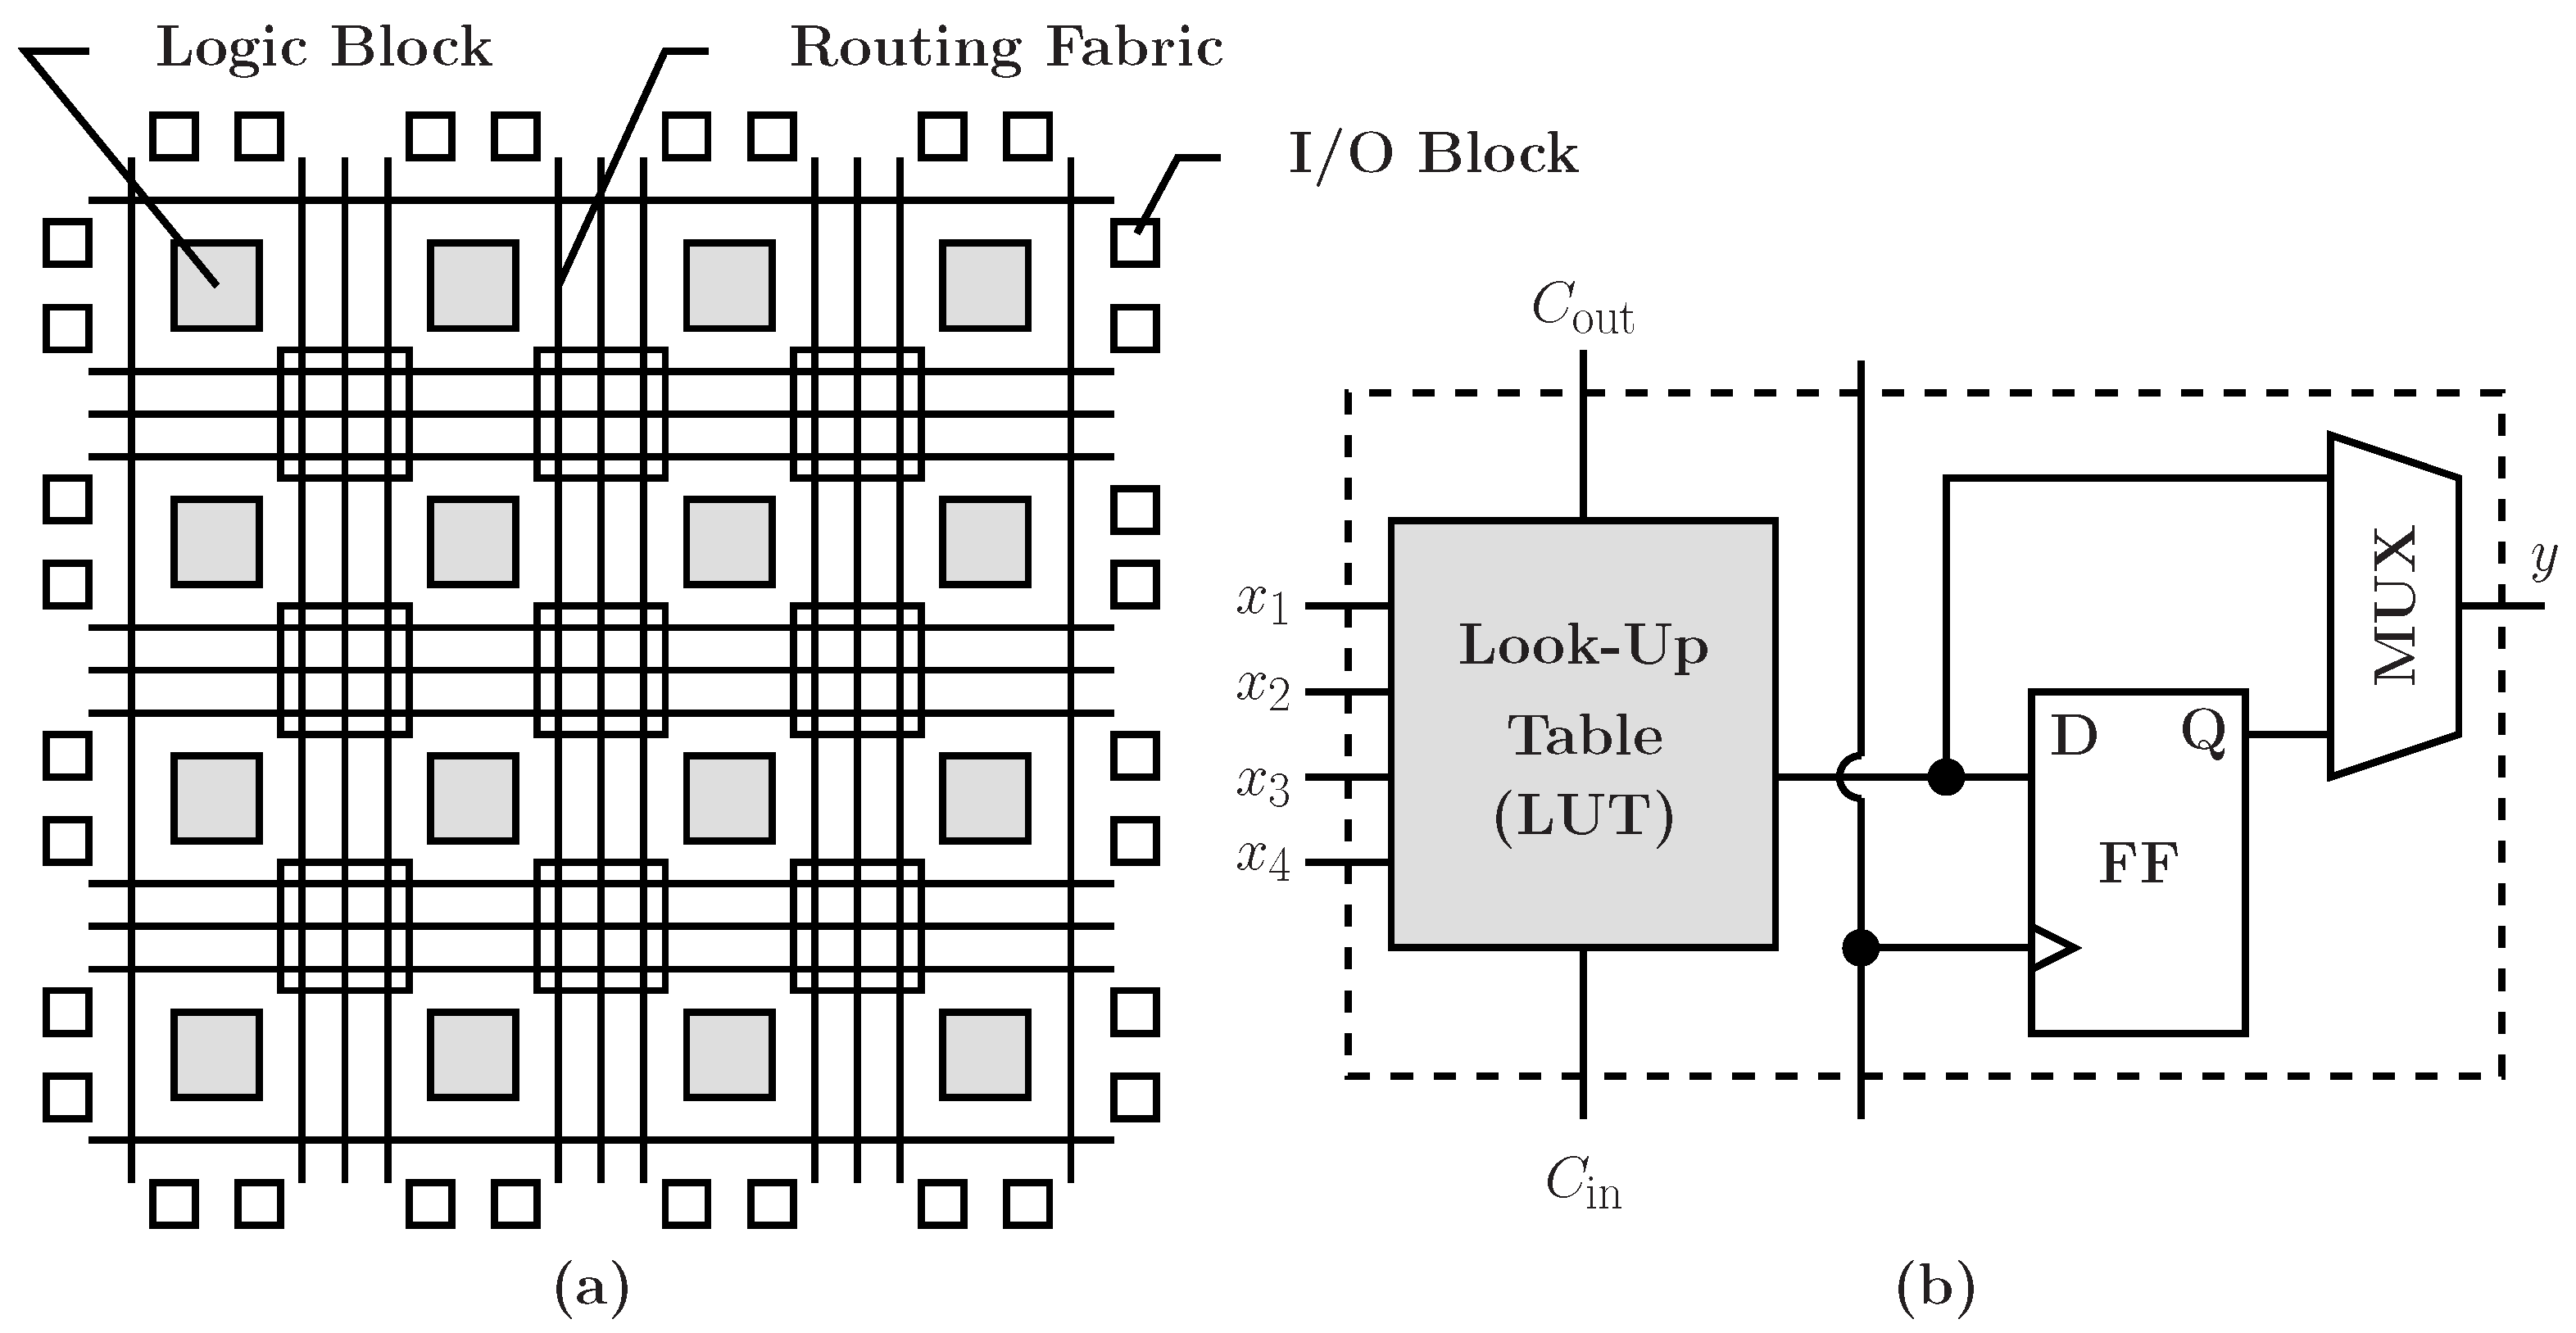
\includegraphics[]{fpga1}
	\caption{Schema FPGA}
\end{figure}

\section{Scrivere e compilare System Verilog}

Creiamo un multiplexer da due bit con System Verilog, compiliamo e visualizziamo con \textbf{GTKWave}

\includecode[verilog]{./verilog/2x1mux/mux.sv}{mux.sv}
\includecode[verilog]{./verilog/2x1mux/test_mux.sv}{test\_mux.sv}

Per compilare, eseguiamo da terminale 
\begin{lstlisting}[style={bash}]
iverilog -g2005-sv nome_sorgente.sv -o nome_eseguibile
\end{lstlisting}

Quindi, per compilare entrambi i file e caricarli in GTKWave:
\begin{lstlisting}[style={bash}]
iverilog -g2005-sv test_mux.sv mux.sv -o test_mux
# Eseguiamo la simulazione
./test_mux
# Viene creato il file provamux.vcd, carichiamolo in GTKWave
gtkwave provamux.vcd &
\end{lstlisting}

\includecode[verilog]{./verilog/2x1mux/mux4.sv}{Multiplexer da 4 vie ad 1 bit}

\includecode[verilog]{./verilog/2x1mux/muxbool.sv}{Multiplexer di variabili booleane}

\clearpage

\section{Esercizi}
\subsection{Automa che riconosce "abba"}

Realizziamo un automa di Mealy che riconosce le stringhe \textit{"abba"} da un insieme $ \{a,b,c\} $. La rete sequenziale dell'automa si realizzerà con i componenti visti in figura ~\ref{fig:mealyautomata1.tex}. Consideriamo la rappresentazione binaria dell'alfabeto con $ a = 00, b = 01, c = 11 $. Per gli stati usiamo la codifica $ S_1 = 00, S_2 = 01, S_3 = 11, S_4 = 10 $

\begin{figure}[H]
	\centering
	\caption{Automa di Mealy che riconosce "abba"}
	\begin{tikzpicture}[->,>=stealth',shorten >=1pt,auto,node distance=3.5cm]
	
	\node[state,accepting] 	(A)                    {$S_1$};
	\node[state]         	(B) [above right of=A] 	   {$S_2$};
	\node[state]         	(C) [below right of=B] 	   {$S_3$};
	\node[state]         	(D) [below right of=A] 	   {$S_4$};
	
	\path 	(A)		edge [bend left]  	node {$a/0$} 		(B)
	edge [loop left] 	node {$b,c/0$} 		(A)
	(B) 	edge [loop above] 	node {$a/0$} 		(B)
	edge [bend left] 	node {$c/0$} 		(A)
	edge [bend left]  	node {$b/0$} 		(C)
	(C)		edge [bend left]  	node {$c/0$} 		(A)
	edge [bend left]  	node {$a/0$} 		(B)
	edge [bend left]  	node {$b/0$} 		(D)
	(D)		edge [bend left]  	node {$b,c/0$} 		(A);
	\end{tikzpicture}
\end{figure}

\begin{table}[H]
	\centering
	\caption{Tabella di verità dell'output della rete sequenziale dell'automa "abba" ($ \omega $)}
	\label{tab:mealyomega2}
	\begin{tabular}{l|llll|l|}
		\cline{2-6}
		& $s_1$ & $s_2$ & $x_1$ & $x_2$ & z \\ \cline{2-6} 
		Stato $S_1$ & 0     & 0     & -     & -     & 0 \\
		Stato $S_2$ & 0     & 1     & -     & -     & 0 \\
		Stato $S_3$ & 1     & 1     & -     & -     & 0 \\
		Stato $S_4$ & 1     & 0     & 0     & 0     & 1 \\
		& 1     & 0     & 0     & 1     & 0 \\
		& 1     & 0     & 1     & 1     & 0 \\ \cline{2-6} 
	\end{tabular}
\end{table}

\begin{table}[H]
	\centering
	\caption{Tabella di verità del cambio di stato dell'automa per riconoscere "abba" ($\sigma$)}
	\label{tab:mealysigma2}
	\begin{tabular}{l|llll|ll|}
		\cline{2-7}
		& $s_1$ & $s_2$ & $x_1$ & $x_2$ & $s_1'$ & $s_2'$ \\ \cline{2-7} 
		Stato $S_1$ & 0     & 0     & 0     & 0     & 0      & 1      \\
		& 0     & 0     & 0     & 1     & 0      & 0      \\
		& 0     & 0     & 1     & 1     & 0      & 0      \\ \cline{2-7} 
		Stato $S_2$ & 0     & 1     & 0     & 0     & 0      & 1      \\
		& 0     & 1     & 0     & 1     & 1      & 1      \\
		& 0     & 1     & 1     & 1     & 0      & 0      \\ \cline{2-7} 
		Stato $S_3$ & 1     & 1     & 0     & 0     & 0      & 1      \\
		& 1     & 1     & 0     & 1     & 1      & 0      \\
		& 1     & 1     & 1     & 1     & 0      & 0      \\ \cline{2-7} 
		Stato $S_4$ & 1     & 0     & 0     & 0     & 0      & 0      \\
		& 1     & 0     & 0     & 1     & 0      & 0      \\
		& 1     & 0     & 1     & 1     & 0      & 0      \\ \cline{2-7} 
	\end{tabular}
\end{table}

% TODO mappa di karnaugh di s1 e s2

Avremo che la formula booleana sarà per il primo e secondo bit di stato:
\[ s_1' = \overbar{s_1}s_2\overbar{x_1}x_2 + s_1s_2\overbar{x_1}x_2 = s_2\overbar{x_1}x_2 \]. 
\[ s_2' = \overbar{s_1s_2}+ \overbar{s_1}s_2\overbar{x_1} + s_2\overbar{x_2}\]

La formula per l'uscita sarà $ z = s_1\overbar{s_2x_1x_2} $. Ci rimane da definire il registro da 2 bit per definire tutta la rete sequenziale. Abbiamo supposto che la rete sequenziale funzioni ricevendo un segnale di clock ad intervalli regolari.
La rete di output $ \omega $ è definita utilizzando soltanto AND ed impiegherà $ \Delta t $ per eseguire l'operazione. La funzione di cambio di stato $ \sigma $ è definita invece con 1 AND e 1 OR ed impiegherà $ 2\Delta t $ per l'operazione.
Il ciclo di clock dev'essere almeno $ \tau = \delta + \max\{t_{\sigma}, t_{\omega}\} $ dove $ \delta $ è la durata del segnale HIGH nel clock.

Abbiamo 3 moduli. Uno per il registro, uno per il modulo $ \omega $ e uno per il modulo $ \sigma $. Scriviamolo in Verilog.

\paragraph{Note}

La sintassi \verb|[a:b]| denota un array indicizzato dal numero \verb|a| al numero \verb|b|. Utilizziamo gli array per rappresentare valori a più bit. In questo caso, il registro è generalizzato per un parametro \verb|N| e può ad esempio essere inizializzato con \verb|registro #(4) nome(...) | dove 4 è il parametro \verb|N| e corrisponde al numero di bit del registro.

La negazione con \verb|!| nega un singolo valore, mentre la notazione \verb|~| viene detta negazione \textit{bit wise} e nega tutti i valori di una sequenza di bit.

Normalmente, in un blocco \verb|assign| assegno un valore ad una variabile booleana istantaneamente. Posso invece aggiungere un delay inserendo \verb|#x| di fronte all'identificatore della variabile, dove \verb|x| è un numero. Ad esempio:
\begin{lstlisting}[style={verilog}]
assign 
	#1 z = (ic == 0 ? x : y)
\end{lstlisting}

\includecode[verilog]{./verilog/abba/Registro/reg.v}{Registro a N bit}
\includecode[verilog]{./verilog/abba/Mealy/sigma.v}{Modulo di $ \sigma $ o funzione di cambio di stato}
\includecode[verilog]{./verilog/abba/Mealy/omega.v}{Modulo di $ \omega $}
\includecode[verilog]{./verilog/abba/Mealy/m1.v}{Modulo della rete sequenziale}
\includecode[verilog]{./verilog/abba/Mealy/test-m1.v}{Modulo di test della rete sequenziale}

\clearpage

\subsection{Automa di Moore per riconoscere "abba"}
Vediamo adesso un automa di Moore per riconoscere la stringa \textit{"abba"} nell'alfabeto $ \{a,b,c\} $. La differenza sta nel fatto che i singoli nodi non hanno accesso all'input $ x $.

\begin{figure}
	\centering
	\caption{Automa di Moore che riconosce "abba"}
	\begin{tikzpicture}[->,>=stealth',shorten >=1pt,auto,node distance=3.5cm]
	
	\node[state,initial] 	(A)                    {$\dfrac{S_1}{0}$};
	\node[state]         	(B) [right of=A] 	   {$\dfrac{S_2}{0}$};
	\node[state]         	(C) [below of=A] 	   {$\dfrac{S_3}{0}$};
	\node[state]         	(D) [below of=B] 	   {$\dfrac{S_4}{0}$};
	\node[state,accepting]  (E) [above right of=D] 	   {$\dfrac{S_4}{0}$};
	
	\path 	(A)		edge [bend left=60]  				node {$a$} 		(B)
					edge [loop above] 					node {$b,c$} 	(A)
			(B) 	edge [loop above] 					node {$a$} 		(B)
					edge [] 							node {$c$} 		(A)
					edge [bend left=20]  				node {$b$} 		(C)
			(C)		edge []  							node {$c$} 		(A)
					edge [bend left=20]  				node {$a$} 		(B)
					edge []  							node {$b$} 		(D)
			(D)		edge [bend left=90,looseness=2]		node {$b,c$} 	(A)
					edge []								node {$a$}		(E)
			(E)		edge [bend right=90,looseness=1.8]  	node {$b,c$} 	(A)
					edge []	node {$a$}		(B);
	\end{tikzpicture}
\end{figure}

\includecode[verilog]{./verilog/abba/Moore/mo-sigma.v}{Modulo di $ \sigma $ o funzione di cambio di stato (Moore)}
\includecode[verilog]{./verilog/abba/Moore/mo-omega.v}{Modulo di $ \omega $ (Moore)}
\includecode[verilog]{./verilog/abba/Moore/moore.v}{Modulo della rete sequenziale (Moore)}
\includecode[verilog]{./verilog/abba/Moore/test-m1.v}{Modulo di test della rete sequenziale (Moore)}
\includecode[makefile]{./verilog/abba/Moore/makefile}{Makefile (Moore)}

\FloatBarrier

\subsection{Mealy con Delay $ \equiv $ Moore}

\includecode[verilog]{./verilog/abba/MealyConDelay/reg-delay.v}{Registro a N bit con delay}
\includecode[verilog]{./verilog/abba/MealyConDelay/sigma-delay.v}{Modulo di $ \sigma $ o funzione di cambio di stato (Mealy con Delay)}
\includecode[verilog]{./verilog/abba/MealyConDelay/omega-delay.v}{Modulo di $ \omega $ (Mealy con Delay)}
\includecode[verilog]{./verilog/abba/MealyConDelay/m1-delay.v}{Modulo della rete sequenziale (Mealy con Delay)}
\includecode[verilog]{./verilog/abba/MealyConDelay/test-m1-delay.v}{Modulo di test della rete sequenziale (Mealy con Delay)}
\includecode[makefile]{./verilog/abba/MealyConDelay/makefile}{Makefile (Mealy con Delay)}

Per sincronizzare il modulo della rete sequenziale dell'automa di Mealy mettiamo un registro di fra l'input \verb|x| e le reti sequenziali \verb|sigma| e \verb|omega|